% !TEX root = cha-application.tex
\documentclass[../../main.tex]{subfiles}

\begin{document}

\section{Min-Heap Behavior}

\label{sec:min_heap_dynamics}

In the previous sections, we explained why we use a \textbf{max-heap} during the WFC observation phase. Empty tiles have higher weights than path tiles. So, as path cells have a higher entropy, with a max-heap they are selected first. This allows paths to be generated before the empty tiles occupy the whole grid, removing space for paths.

Standard WFC implementations usually use a \textbf{min-heap}, which selects the cells with the lowest entropy first. In our case, this means that empty tiles are selected before path tiles. This produces an interesting behavior: sometimes, instead of blocking the paths, the empty tiles can help guide them.

\subsection{How Min-Heap Can Guide Paths}

With a min-heap, empty tiles quickly fill the majority of the grid. As more cells become empty, the available space for paths becomes smaller.

The remaining uncollapsed cells form narrow areas between the classes. Since the paths still need to connect the classes, they are forced to use these remaining areas. In this way, the empty tiles naturally guide the paths through the grid.

This behavior allows min-heap to succeed in generating a solution even without path boost, that we showed is really important in \secref{sec:path_boost_effect}.

\subsection{Example: Slot Hierarchy}

To show this behavior, we use the complete class hierarchy of the \texttt{Slot} class in Pharo 13. The system contains 30 classes, which were placed on a $34 \times 34$ grid. 

The generation took 14~minutes and 54~seconds and required 1,139 retries. Figure~\ref{fig:min_heap_comparison} shows an intermediate step and the final result.

\begin{figure}[ht]
    \centering
    \begin{subfigure}[b]{0.48\textwidth}
        \centering
        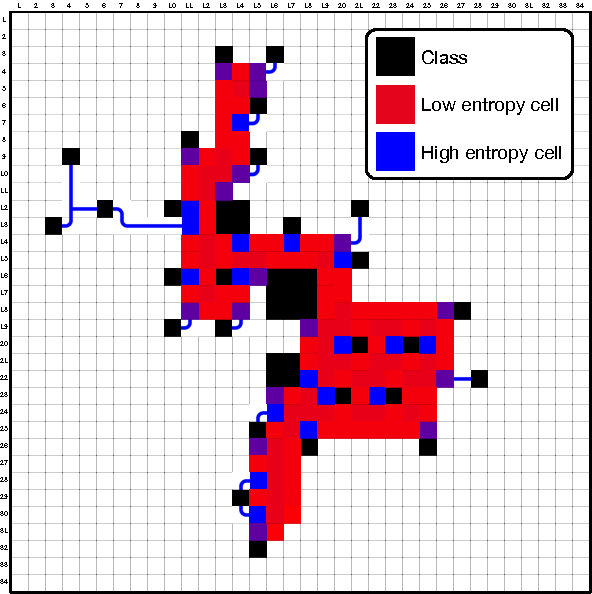
\includegraphics[width=\textwidth]{figures/application/min_heap_step_1006}
        \caption{Step 1006 / 1156 (87\% complete).}
        \label{fig:min_heap_step}
    \end{subfigure}
    \hfill
    \begin{subfigure}[b]{0.48\textwidth}
        \centering
        \includegraphics[width=\textwidth]{figures/application/min_heap_final}
        \caption{Final visualization (Step 1156).}
        \label{fig:min_heap_final}
    \end{subfigure}
    \caption{Min-heap generation process.}
    \label{fig:min_heap_comparison}
\end{figure}

In Figure~\ref{fig:min_heap_step}, most of the grid has already been filled with empty tiles, shown as white areas. This leaves only uncollapsed cells between the classes. These remaining cells form narrow corridors that guide the paths. Figure~\ref{fig:min_heap_final} shows the result, where the paths have followed these remaining areas and successfully connected all classes.

\end{document}